\documentclass{article}
\usepackage{hyperref}
\usepackage[utf8]{inputenc}
\usepackage[margin=12.7mm]{geometry}
\usepackage{helvet}
\usepackage{graphicx}
\usepackage{color}
\usepackage[parfill]{parskip}
\usepackage{titlesec}
\titleformat*{\section}{\LARGE\bfseries}
\titleformat*{\subsection}{\Large\bfseries}
\graphicspath{ {./images/} }

\renewcommand{\familydefault}{\sfdefault}
\author{G12}
\title{Documento di architettura}
\date{}
\begin{document}
      \maketitle 
      \tableofcontents
      \clearpage
      \section{Scopo del documento}
      Il presente documento riporta la definizione dell’architettura del progetto SmartFit. Verrà utilizzato un diagramma delle classi in Unified
      Modeling Language (UML) e del codice in Object Constraint Language (OCL) per esprimere in modo formale e privo di ambiguità le regole che
      vengono applicate al diagramma in UML. Nel precedente documento era stata progettata l’architettura del progetto mediante diagrammi di
      contesto, dei componenti e Business Process Model and Notation (BPMN). In questo documento, invece, facendo riferimento alla progettazione
      fatta, viene definita l’architettura del sistema elencando e descrivendo le varie classi e interfacce che dovranno essere implementate, con
      anche i vari collegamenti tra di esse. Inoltre, verrà descritta la logica che regola il comportamento del software con l’utilizzo di OCL per
      tali concetti e regole che non possono in alcun modo essere espressi all’interno del Class Diagram.\\

      \section{Diagramma delle classi}
      Nel presente capitolo vengono elencate e descritte le varie classi previste nel progetto SmartFit. In riferimento al documento di progettazione
      dell’architettura, ogni sistema esterno e attore presente nel diagramma di contesto, e ogni componente presente nel diagramma dei componenti
      diverranno una o più classi in questo documento di definizione dell’architettura. Le varie classi potranno anche eventualmente essere associate
      ad altre descrivendo, se necessario, informazioni aggiuntive per quanto riguarda la relazione tra di esse.\\


      Si riportano ora le varie classi individuate a partire dai diagrammi di progettazione dell’architettura presenti nel precedente documento.
      In questa procedura si è tentato di massimizzare il livello di coesione tra le varie classi anche se a volte però si è dovuto fare qualche
      sacrificio per l’impossibilità di rappresentare in UML determinati concetti. Si è quindi preferito procedere con un’accurata descrizione
      delle scelte di definizione dell’architettura per poi descrivere in codice OCL i vari vincoli che vertono nelle e tra le classi descritte.
      Per le varie classi si è anche deciso di fornire una breve descrizione di alcune funzioni e attributi nel caso in cui il nome non fosse autoesplicativo.\\


      Prima di tutto, andiamo a descrivere alcuni tipi di dato che abbiamo dovuto introdurre per trattare determinati dati utilizzati
      dall’applicazione.\\

      \subsection{Tipi di dato}
      {\large\textbf{Pasto}}\\

      L’utente può inserire i suoi pasti assunti quindi è stato necessario creare un tipo di dato “Pasto” che possa descrivere tali oggetti. Questo tipo di dato verrà utilizzato sia nelle liste giornaliere dei pasti assunti dall’utente sia per la sua cronologia e andamento.\\
      \begin{center}
            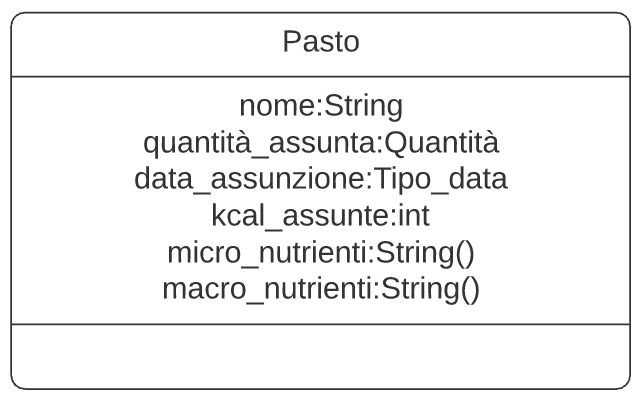
\includegraphics[scale=0.5]{images/classi/Pasto.png}
      \end{center}
      {\large\textbf{Attività}}\\

      L’utente può inserire le sue attività svolte quindi è stato necessario creare un tipo di dato “Attività” che possa descrivere tali oggetti. Questo tipo di dato verrà utilizzato sia nelle liste giornaliere delle attività svolte dall’utente sia per la sua cronologia e andamento.\\
      \begin{center}
            \includegraphics[scale=0.5]{classi/Attività.png}

            
      \end{center}

      {\large\textbf{Unità di misura}}\\

      Abbiamo individuato il tipo unità di misura "Tipo\_unità\_di\_misura", Questo tipo è una semplice enumerazione con due valori, che sono
      relativamente kg/m e lb/ft. Abbiamo preferito utilizzare un’enumerazione come questa perché oltre a rendere più chiaro il diagramma delle
      classi e di conseguenza il codice che verrà prodotto, semplifica di molto anche la modifica se si volesse aggiungere qualsiasi altra unità.
      Questo tipo di dato viene utilizzato dalla classe "Utente" (descritta successivamente) per salvare la preferenza dell’unità di misura da
      utilizzare all’interno dell’app. Viene inoltre utilizzata da una funzione che va a convertire tutti i dati salvati in accordo con l’unità di
      misura scelta, presente nella classe “Gestione\_profilo\_utente” descritta successivamente.\\
      \begin{center}
            \includegraphics[scale=0.5]{classi/Tipo_unità_di_misura.png}
      \end{center}

      {\large\textbf{Quantità}}\\

      Abbiamo individuato il tipo "Quantità". Questo tipo è una semplice enumerazione con 6 valori. Questo tipo di dato verrà utilizzato per
      permettere all’utente di inserire la quantità assunta di un determinato alimento, il quale può essere sia solido che liquido.\\
      \begin{center}
            \includegraphics[scale=0.5]{classi/Quantità.png}
      \end{center}

      {\large\textbf{Tempo}}\\

      Abbiamo individuato un tipo di dato che va a salvare il tempo "Tipo\_tempo", espresso in ore, minuti e secondi. Questa è una semplice classe
      con i sopracitati attributi. La suddetta classe viene utilizzata ad esempio per salvare la durata di un’attività fisica o anche in un altro
      tipo di dato che ora sarà descritto.\\
      \begin{center}
            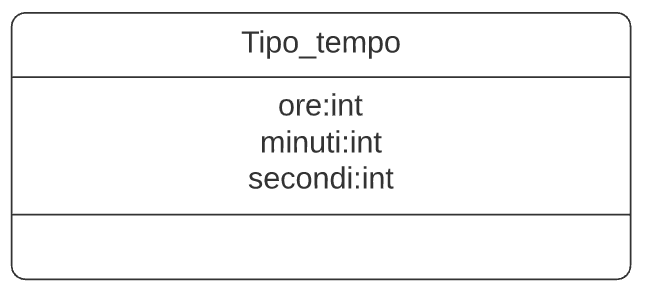
\includegraphics[scale=0.5]{classi/Tipo_tempo.png}
      \end{center}
      
      \hfill \break

      {\large\textbf{Data}}\\

      Abbiamo individuato un tipo di dato che va a salvare la data "Tipo\_data". Questa semplice classe contiene gli attributi anno, mese, giorno e
      inoltre l’ora (salvata con il tipo di dato "Tipo\_tempo" appena descritto). La suddetta classe viene utilizzata per mantenere in ordine
      cronologico il riepilogo dei pasti e attività dell’utente. Viene in utilizzata per tenere la cronologia dell’utente, sapere quando sono passati i 14 giorni
      dopo i quali si può eliminare un determinato elemento dalla cronologia o le 24 ore per il blocco momentaneo dell’accesso. Ovviamente tutte
      queste funzionalità verranno descritte successivamente.\\
      \begin{center}
            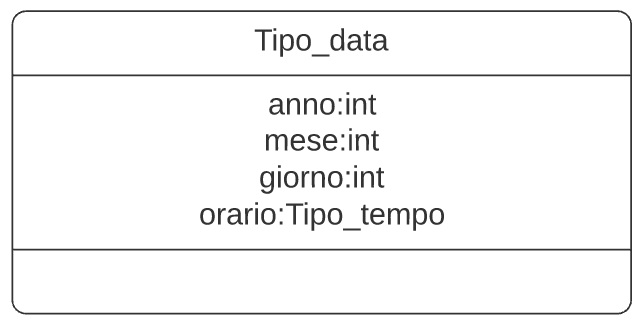
\includegraphics[scale=0.5]{classi/Tipo_data.png}
      \end{center}

      {\large\textbf{Lingua}}\\

      Abbiamo individuato un tipo di dato che va a salvare la lingua di sistema "Tipo\_lingua". Anche in questo caso si è deciso di optare per una
      semplice enumerazione con solo la lingua italiana e inglese per i medesimi motivi dell’enumerazione delle unità di misura. Questo tipo di
      dato verrà utilizzato dall’applicazione per salvare all’avvio dell’app la lingua per poi selezionare correttamente il language pack da
      utilizzare.\\
      \begin{center}
            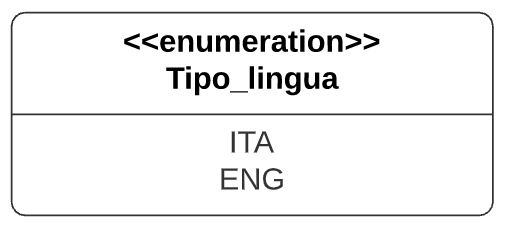
\includegraphics[scale=0.5]{classi/Tipo_lingua.png}
      \end{center}

      \subsection{Classi funzionali}
      Si procede ora con la descrizione di certe classi la cui funzione è di raccogliere, o raggruppare, metodi riguardanti funzionalità cardine
      utilizzate da più classi. È stato deciso di utilizzare questo tipo di classe per massimizzare il livello di accoppiamento laddove non ci
      eravamo riusciti nel diagramma dei componenti senza complicarlo troppo portando quindi a certi componenti di livello informazionale anziché
      funzionale. Le classi sono astratte e tutte le funzioni contenute ovviamente devono essere statiche dato che la classe essendo astratta non
      può essere istanziata. Questa scelta è stata presa perché non avrebbe senso voler creare istanze di queste classi dato che le funzioni non
      agiscono direttamente su altre classi bensì forniscono informazioni oppure svolgono funzioni molto specifiche e non legate ad altri oggetti.\\ 


      {\large\textbf{Comunicazione con il sistema operativo}}\\

      La classe astratta "Comunicazione\_sistema\_operativo" contiene tutti i vari metodi che permettono di interfacciarsi con il sistema operativo
      (Android) su cui l’applicazione è in esecuzione. Le funzioni contenute permettono di avere informazioni sullo stato del sistema o accedere a
      file interni o al sistema di gestione notifiche push.\\
      \begin{center}
            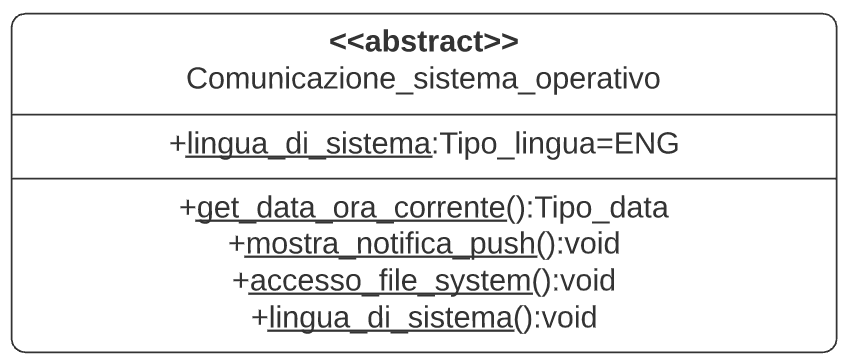
\includegraphics[scale=0.5]{classi/Comunicazione_sistema_operativo.png}
      \end{center}


      {\large\textbf{Gestione notifiche}}\\

      La classe astratta "Gestione\_notifiche" gestisce le notifiche interne all’applicazione. Le varie funzioni vengono semplicemente chiamate
      quando si vuole mostrare la relativa notifica nell’applicazione dell’utente.\\
      \begin{center}
            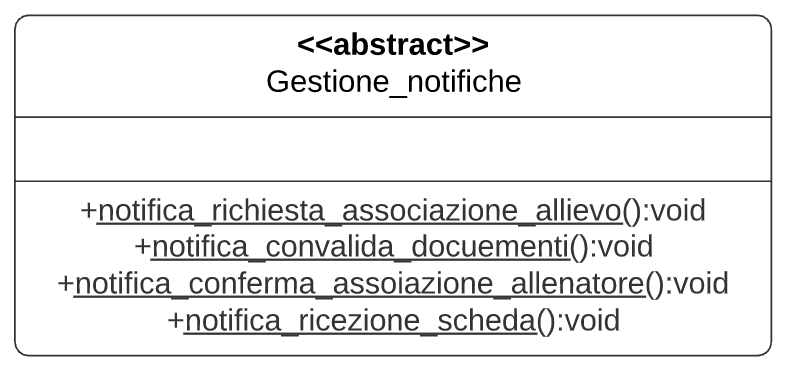
\includegraphics[scale=0.5]{classi/Gestione_notifiche.png}
      \end{center}

      {\large\textbf{Utilities sicurezza}}\\

      La classe astratta "Utilities\_sicurezza" è stata creata per gestire una funzionalità che non era stato possibile rappresentare nello scorso
      documento. Nel documento delle specifiche dei requisiti, nei requisiti non funzionali era richiesto un buon livello di sicurezza per quanto
      riguardava le credenziali di accesso. Dato che l’utente può scegliere di salvare le credenziali nel dispositivo per non doverle inserire a
      ogni accesso, si è pensato di non solo memorizzarle criptate ma anche utilizzarle criptate all’interno dell’applicazione in modo da non
      renderla visibile ad attacchi come il core dump. In questo modo la funzione di criptazione della password verrà utilizzata quando si va a
      inserirla per la prima volta o quando se ne inserisce una nuova. La funzione di decrittazione invece viene utilizzata ogni qual volta che
      bisogna utilizzare le credenziali per autenticarsi con il database esterno (la connessione ovviamente sarà anch’essa criptata).\\
      \begin{center}
            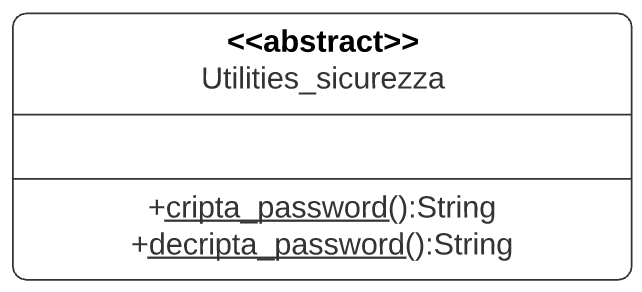
\includegraphics[scale=0.5]{classi/Utilities_sicurezza.png}
      \end{center}

      \subsection{Classi individuate da contesto e componenti}
      Seguono ora le classi derivate dall’analisi del contesto e dei componenti dello scorso documento.\\


      {\large\textbf{Utenti}}\\

      Visionando l’analisi del contesto dello scorso documento si può notare che ci sono due attori, “Utente” e “Allenatore”. Purtroppo non è
      stato possibile rappresentare in UML questi due tipi di account. C’erano troppi fattori che si univano in questo caso per essere gestiti. Un
      utente può diventare un allenatore, un utente può essere un allievo di un allenatore ma anche un allenatore può allenare un allenatore e
      quindi di conseguenza pure un allenatore può essere un allievo. Questo ha portato alla creazione di una classe “Utente” che comprende già la
      possibilità per un utente di diventare e cessare di essere un allievo e anche di diventare un allenatore, oltre che permette a un allenatore
      di avere un altro allenatore. Per poter regolare il tutto, e non permettere ad esempio a un utente normale di accedere a funzioni riservate a
      un allenatore si è deciso di procedere aggiungendo un attributo booleano “is\_Allenatore” e le relazioni con altre classi faranno quindi
      riferimento a questo parametro come verrà anche descritto in OCL.
      Le varie funzioni "get\_*()" che sono state specificate nella classe Utente sono quelle che possono essere utilizzate solo da un allenatore su
      un suo allievo o da parte di un utente riguardo il proprio allenatore, come poi verrà specificato in OCL.
      L'utente può anche avere, come attributo, i suoi documenti personali di allenatore. I documenti sono un artefatto "documenti\_allenatore.pdf" che è il file pdf contenente i documenti standard rilasciati da un ente nazionale adibito, i quali comprovano la professione di allenatore.\\
      
      \begin{center}
            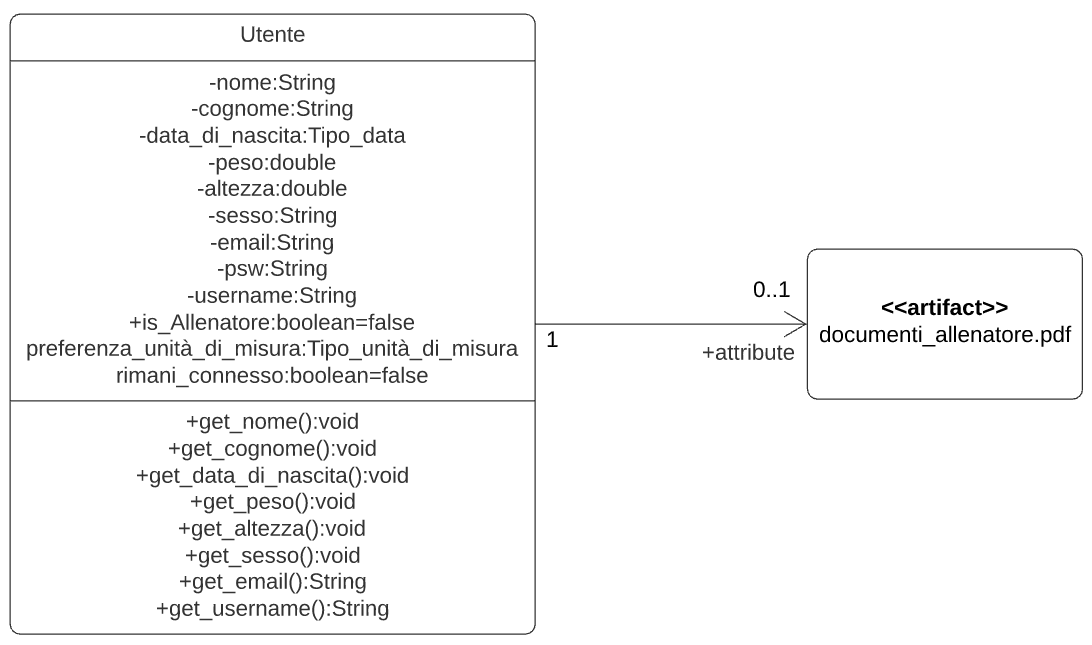
\includegraphics[scale=0.5]{classi/Utente.png}
      \end{center}
      

      {\large\textbf{Sistema di invio email}}\\

      Come si era visto nello studio del contesto, l’applicazione utilizza un servizio esterno per inviare delle email, il sistema subordinato "Sistema di invio email". Dallo studio dei componenti era emerso che fosse necessaria un’interfaccia “Invio email” tra l’applicazione e il sistema esterno. Per questo scopo è stata individuata la classe “Servizio\_invio\_email”. Questa classe fornisce i metodi con cui si possono creare le varie tipologie di email in base al tipo di email da inviare; permette poi di interfacciarsi con il sistema esterno per inviare la email con le informazioni salvate dalle funzioni.\\
      
      \begin{center}
            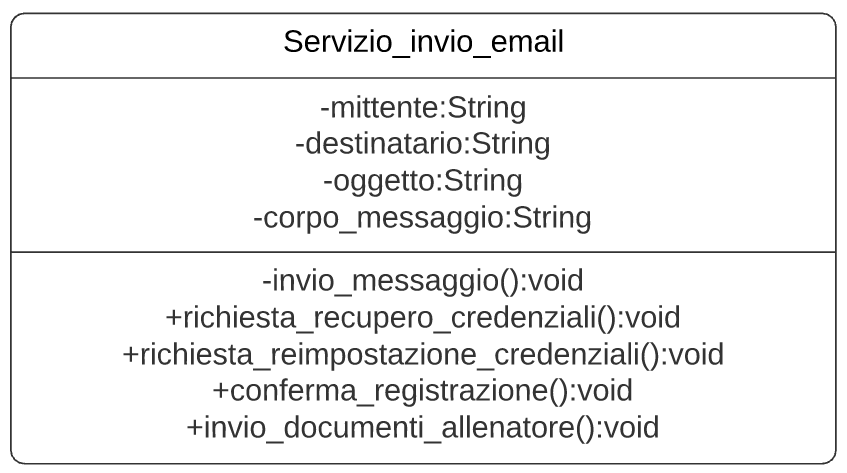
\includegraphics[scale=0.5]{classi/Servizio_invio_email.png}
      \end{center}


      {\large\textbf{Ufficio controllo documenti}}\\

      Nello studio del contesto si può vedere che c’è il sistema subordinato “Ufficio controllo documenti” che si occupa del controllo e convalida dei documenti di un allenatore. Dallo studio dei componenti si era notato che dovesse esserci un’interfaccia “Controllo documenti” con il suddetto sistema esterno. La classe “Controllo\_documenti” gestisce e formula la richiesta per il controllo dei documenti da parte dell’ufficio adibito.\\
      
      \begin{center}
            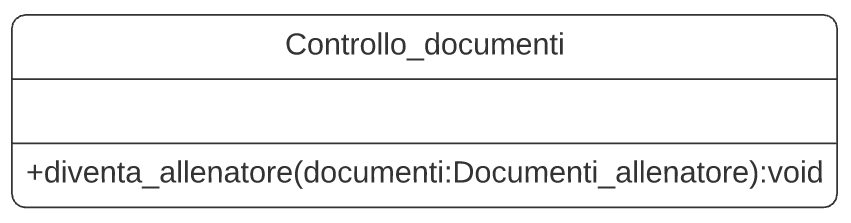
\includegraphics[scale=0.5]{classi/Controllo_documenti.png}
      \end{center}


      {\large\textbf{Database anagrafica utenti}}\\

      Come si era visto nello studio del contesto, l’applicazione utilizza un database esterno per salvare l’anagrafica degli utenti, il sistema subordinato "Database anagrafica utenti". Dallo studio dei componenti era emerso che fosse necessaria un’interfaccia tra l’applicazione e il sistema esterno. Per questo scopo è stata individuata la classe “DB\_anagrafica\_utenti”. Questa classe contiene i metodi che permettono di inviare query al suddetto database, fornite da funzioni di altre classi come si vedrà più avanti. Fornisce anche la funzione con cui si va a controllare se c’è un match con determinate credenziali all’interno del database, funzione che verrà utilizzata sia per la registrazione sia per la modifica delle credenziali da parte dell’utente.\\
      \begin{center}
            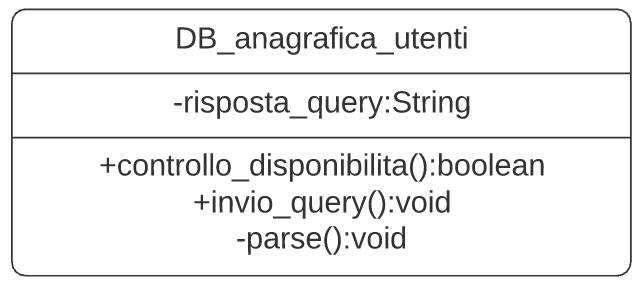
\includegraphics[scale=0.5]{classi/DB_anagrafica_utenti.png}
      \end{center}

      {\large\textbf{Database macro e micro nutrienti per i vari cibi}}\\

      Come si era visto nello studio del contesto, l’applicazione utilizza un database esterno per il calcolo dei micro e macronutrienti dei cibi assunti da un utente, il sistema subordinato "Database macro e micro-nutrienti per i vari cibi". Dallo studio dei componenti era emerso che fosse necessaria un’interfaccia tra l’applicazione e il sistema esterno. Per questo scopo è stata individuata la classe “DB\_nutrienti”. Questa classe contiene i metodi che permettono di inviare query al suddetto database. Le funzioni presenti aiutano la funzione principale “imposta\_valori\_nutrizionali()” a ricavare le varie parti della risposta (micronutrienti, macronutrienti e kcal) da parte del database.\\
      \begin{center}
            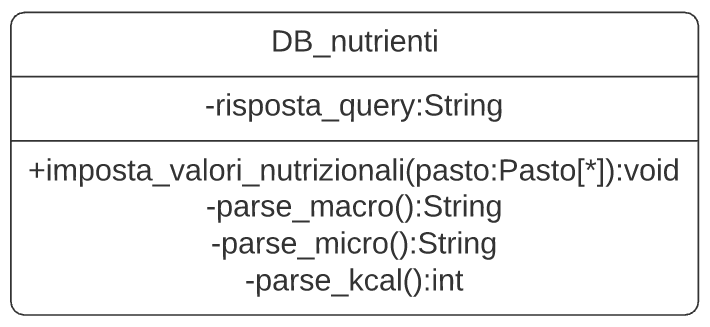
\includegraphics[scale=0.5]{classi/DB_nutrienti.png}
      \end{center}

      {\large\textbf{Dispositivi smart Google}}\\

      L’applicazione utilizza le API di Google per gestire i dispositivi smart di fitness come visto nello studio del contesto, con il sistema subordinato "Dispositivi smart Google". È stata quindi individuata la classe “Gestione\_dispositivi\_smart” che gestisce tutte le varie funzionalità associate a tali dispositivi, quindi l’associazione a essi e la ricezione delle informazioni che collezionano durante l’allenamento dell’utente.\\
      \begin{center}
            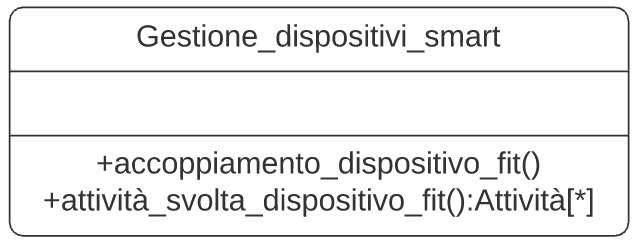
\includegraphics[scale=0.5]{classi/Gestione_dispositivi_smart.png}
      \end{center}

      {\large\textbf{Gestione autenticazione}}\\

      Analizzando il componente “Gestione autenticazione” si è resa necessaria la creazione di una classe “Gestione\_autenticazione” la quale gestisce tutte le varie funzionalità che l’utente può utilizzare all’accesso dell’app. Le funzioni “mantieni\_accesso()” e “reset\_accesso()” gestiscono la scelta dell’utente di mantenere oppure no salvate le credenziali all’interno dell’app per non doverle ripetere a ogni avvio, come da requisito funzionale. Da requisito non funzionale sulla sicurezza nella specifica dei requisiti, infine, si è resa necessaria l’introduzione di altri metodi per la gestione del blocco dell’account in caso di tre successivi tentativi di accesso, come verrà poi descritto dal codice OCL. Ovviamente è stata quindi aggiunta anche una funzione per sbloccare l’accesso dopo 24 ore.
      Dato che l’utente può decidere di salvare le sue credenziali di accesso all’interno del dispositivo si ha avuto la necessità di aggiungere un artefatto “dati\_utente.txt” che conterrà tali dati, con la password criptata dalla classe “Utilities\_sicurezza” come descritto sopra. È  stato deciso di utilizzare un file plain text e non un file criptato per motivi di successiva complessità di gestione ma questo non va a diminuire la sicurezza dell’app in quanto le informazioni contenute sono cifrate.\\
      
      \begin{center}
            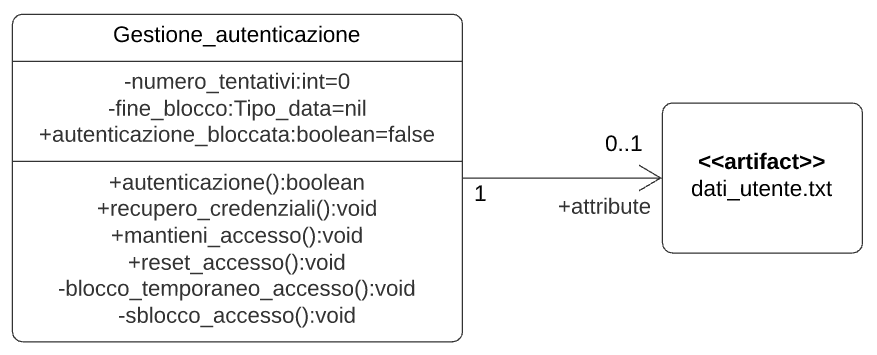
\includegraphics[scale=0.5]{classi/Gestione_autenticazione.png}
      \end{center}
      
      

      {\large\textbf{Gestione registrazione}}\\

      Analizzando il componente “Gestione registrazione” si è resa necessaria la creazione di una classe “Gestione\_registrazione” la quale gestisce la creazione di un nuovo account. Nella sezione di sicurezza dei requisiti non funzionali nella specifica dei requisiti, erano descritte le proprietà che la password deve rispettare per essere accettata. È stata quindi individuata anche una funzione per il controllo che la password inserita sia una strong password per permettere all’utente di continuare con la registrazione o la modifica della password in un secondo momento.\\

      \begin{center}
            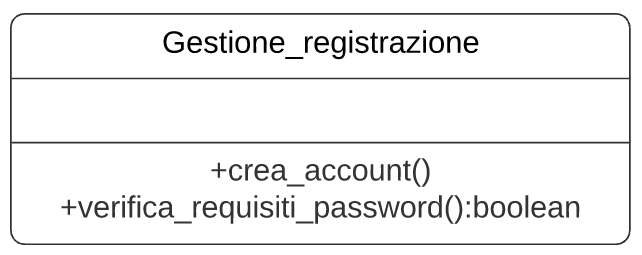
\includegraphics[scale=0.5]{classi/Gestione_registrazione.png}
      \end{center}

      {\large\textbf{Modifica profilo utente}}\\

      Analizzando il componente “Modifica profilo utente” si è resa necessaria la creazione di una classe “Gestione\_profilo\_utente”. Questa classe gestisce tutte le varie funzioni che l’utente ha a disposizione per modificare i suoi dati, che siano i suoi dati biometrici o le credenziali di accesso. È stata anche individuata una funzione “conversione\_unità\_di\_misura()” la quale permette di convertire i vari dati salvati nell’applicazione nel caso in cui l’utente decida di cambiare la sua preferenza sull’unità di misura utilizzata.\\

      \begin{center}
            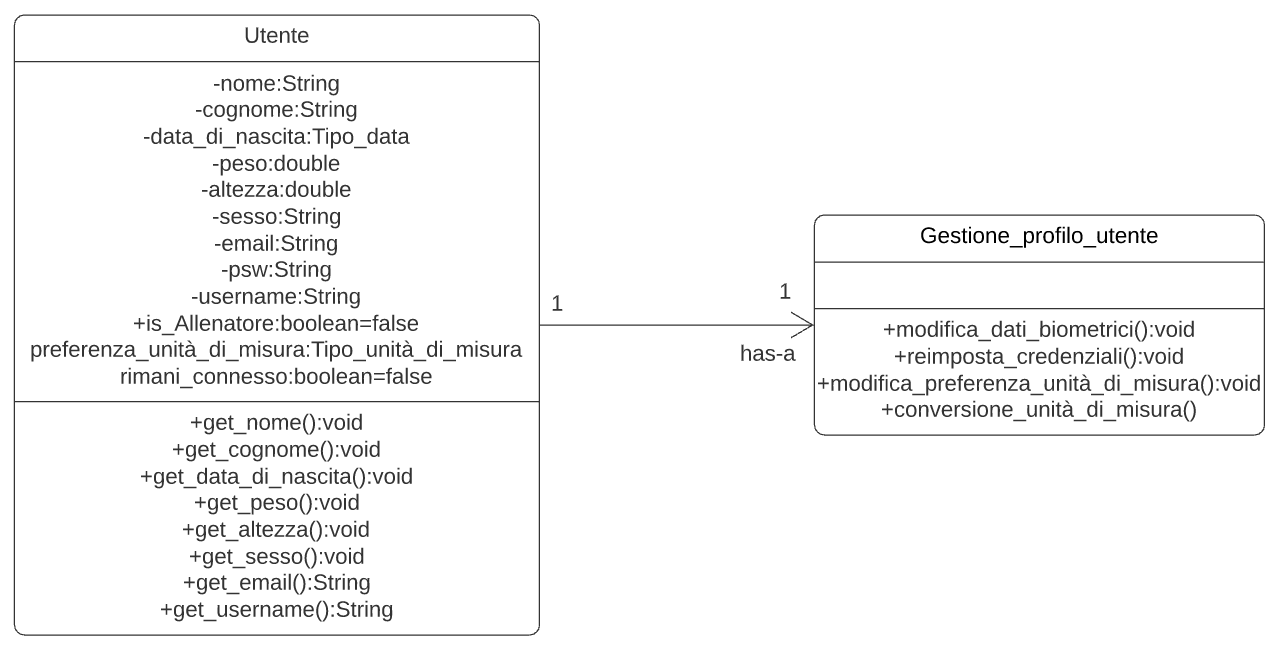
\includegraphics[scale=0.5]{classi/Gestione_profilo_utente.png}
      \end{center}

      {\large\textbf{Gestione allievi}}\\

      Analizzando il componente “Gestione allievi” si è deciso di creare la classe “Gestione\_allievi”. Questa classe è riservata solo agli allenatori, il vincolo verrà descritto in OCL in più avanti. La classe contiene tutte le varie funzioni che un allenatore può utilizzare per interagire con i propri allievi. Si ricorda che l’invio di una scheda, che sia di alimentazione o di allenamento, deve essere eseguito appena dopo la creazione come da specifica dei requisiti. Quindi la funzione “invio\_scheda()”, che invia una determinata scheda ai vari allievi selezionati, dovrà essere chiamata alla fine della procedura di creazione della scheda.
      Si può notare che è necessario il collegamento con i vari artefatti dei file di plain text delle schede. Questo è dovuto al fatto che un allenatore può sempre visualizzare le schede che ha inviato ai suoi allievi anche in secondo momento mentre visualizza le informazioni dei vari allievi. Maggiori informazioni sulla cardinalità sono riportate direttamente nell’immagine sottostante.\\

      \begin{center}
            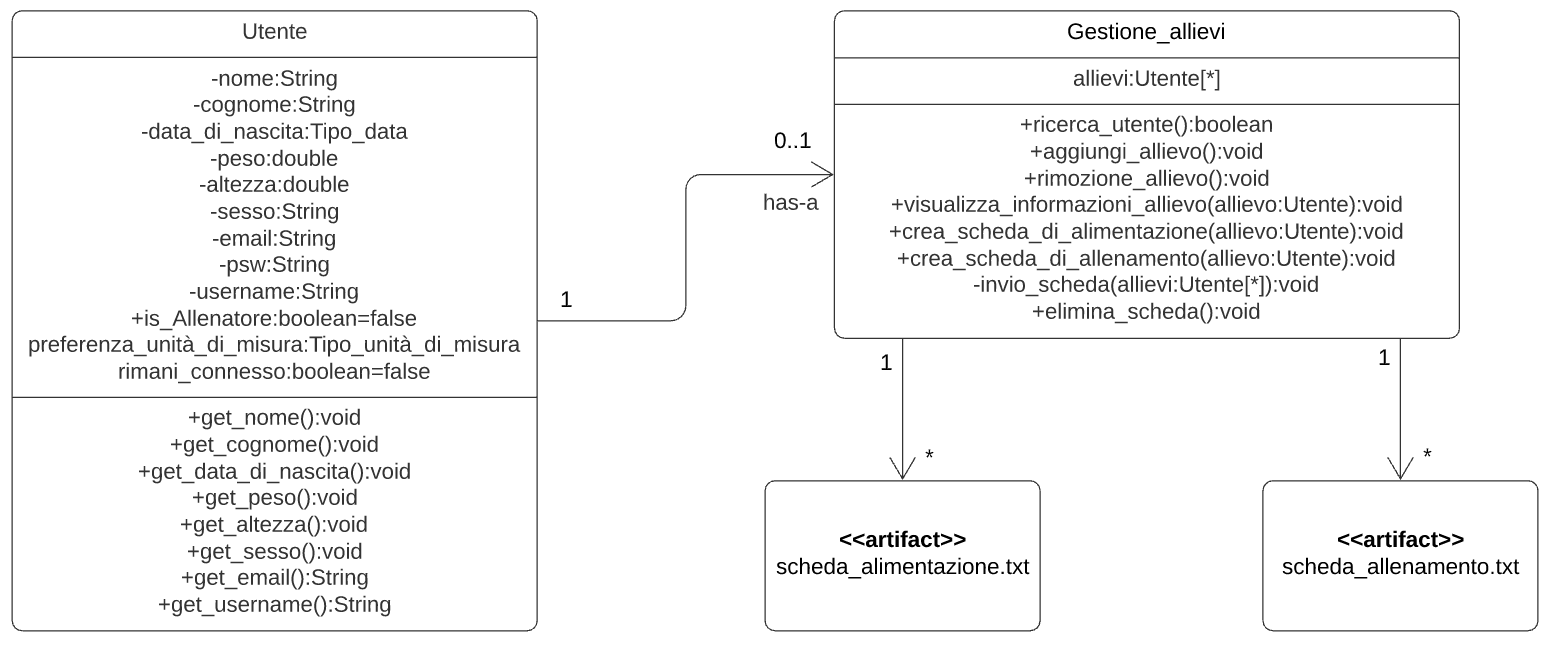
\includegraphics[scale=0.5]{classi/Gestione_allievi.png}
      \end{center}

      {\large\textbf{Gestione allenatore e schede}}\\

      Analizzando il componente “Gestione allenatore e schede” si è deciso di creare la classe “Gestione\_allenatore\_schede”. Questa classe contiene tutte le funzioni che permettono all’utente di gestire il suo legame con il suo allenatore e le schede che esso gli invia. La classe è in relazione uno a uno con la classe Utente, questo perché gestisce anche l’associazione con un allenatore quindi ci deve essere anche quando l’utente non è ancora un allievo, le funzioni devono essere quindi implementate in modo da evitare errori in questa eventualità, come verrà poi descritto anche in OCL.
      Come si può notare la classe ha 2 artefatti, sono i file di plain text delle schede personalizzate dell’utente. Ovviamente un determinato utente può averne o 0 o 1 di ambedue le schede dato che dipende se il suo allenatore gliele ha inviate. Maggiori informazioni sulla cardinalità sono riportate direttamente nell’immagine sottostante. La funzione “init\_schede()” è solo una funzione per l’inizializzazione delle stringhe con le schede all’avvio dell’app. Decisione presa per mantenere una maggiore fluidità dell’applicazione senza dover aprire costantemente degli stream di ingresso ogni qualvolta l’utente vuole visionare le sue schede personalizzate. In questo modo è stata garantita una fruibilità migliore dell’applicazione come era stato richiesto nei requisiti non funzionali della specifica dei requisiti.\\

      \begin{center}
            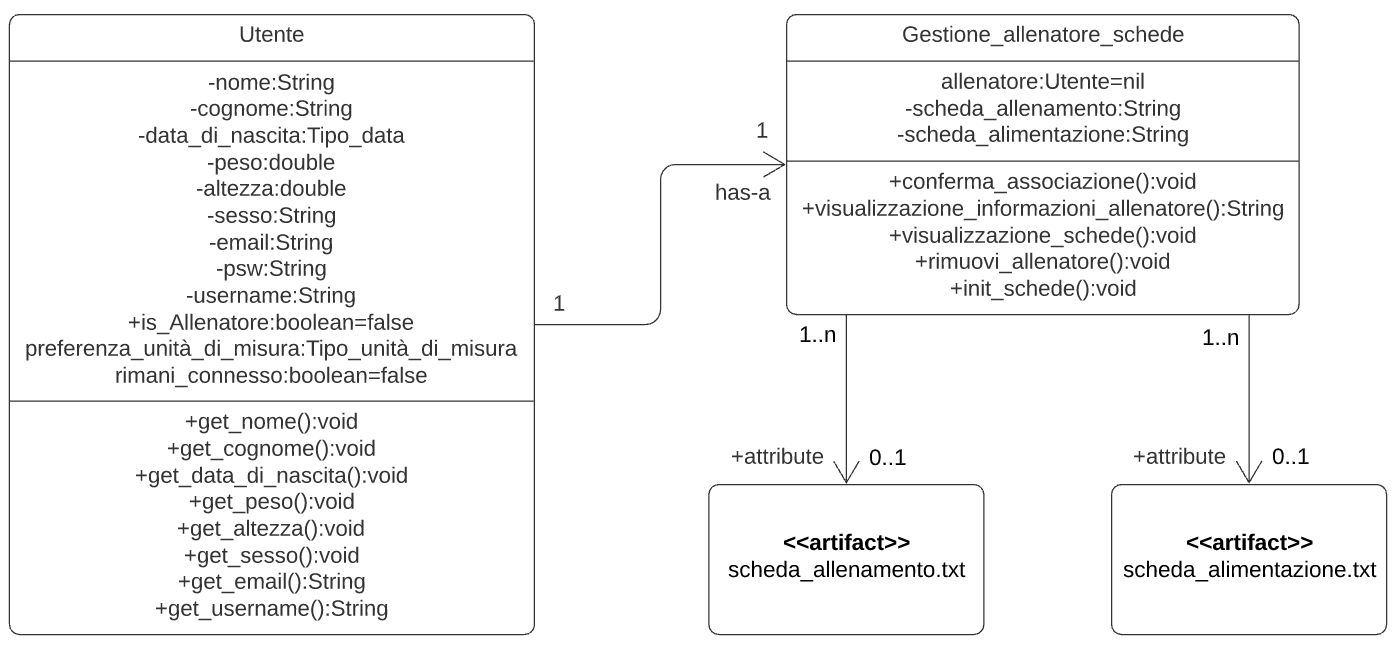
\includegraphics[scale=0.5]{classi/Gestione_allenatore_schede.png}
      \end{center}

      {\large\textbf{Andamento utente}}\\

      Nello studio dei componenti era stato individuato il componente “Andamento utente”. È stata individuata la classe “Andamento\_utente” che contiene tutte le funzioni che riguardano la cronologia di pasti consumati e attività svolte da parte di un determinato utente. Le varie funzioni di sincronizzazione vengono utilizzate per sincronizzare le liste presenti in questa classe con gli elementi presenti nei riepiloghi giornalieri all’interno delle classi di gestione dieta e allenamento dell’utente, che verranno descritte a breve. La funzione “elimina\_elementi\_passati()” serve per eliminare quegli elementi nelle liste di cronologia che sono presenti da più di 14 giorni.
      Le liste di cronologia vengono anche salvate all’interno di artefatti, nello specifico due file di plain text per poter mantenere la cronologia anche a istanze diverse dell’app. La funzione “init\_cronologie()” è equivalente a quella descritta per la classe “Gestione\_allenatore\_schede”.\\

      \begin{center}
            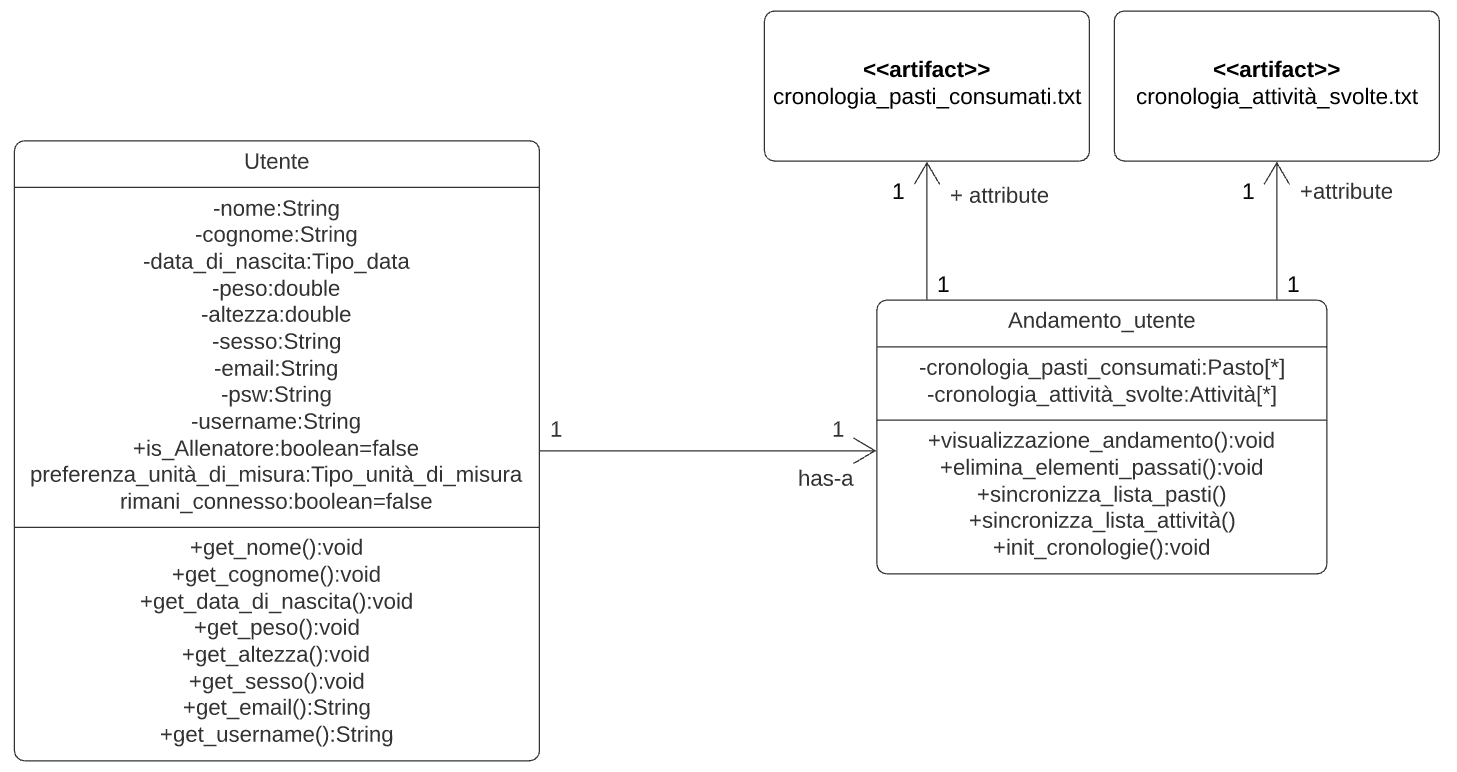
\includegraphics[scale=0.5]{classi/Andamento_utente.png}
      \end{center}

      {\large\textbf{Gestione dieta}}\\

      Nello studio dei componenti era stato individuato il componente “Gestione dieta”. È stata quindi creata la classe “Gestione\_dieta” che contiene tutte le funzioni che vanno a gestire la dieta dell’utente con il relativo andamento giornaliero. La funzione “reset\_list()” viene utilizzata per svuotare la lista allo scadere della mezzanotte dato che la lista è giornaliera e la cronologia viene tenuta nella classe “Andamento\_utente”.\\

      \begin{center}
            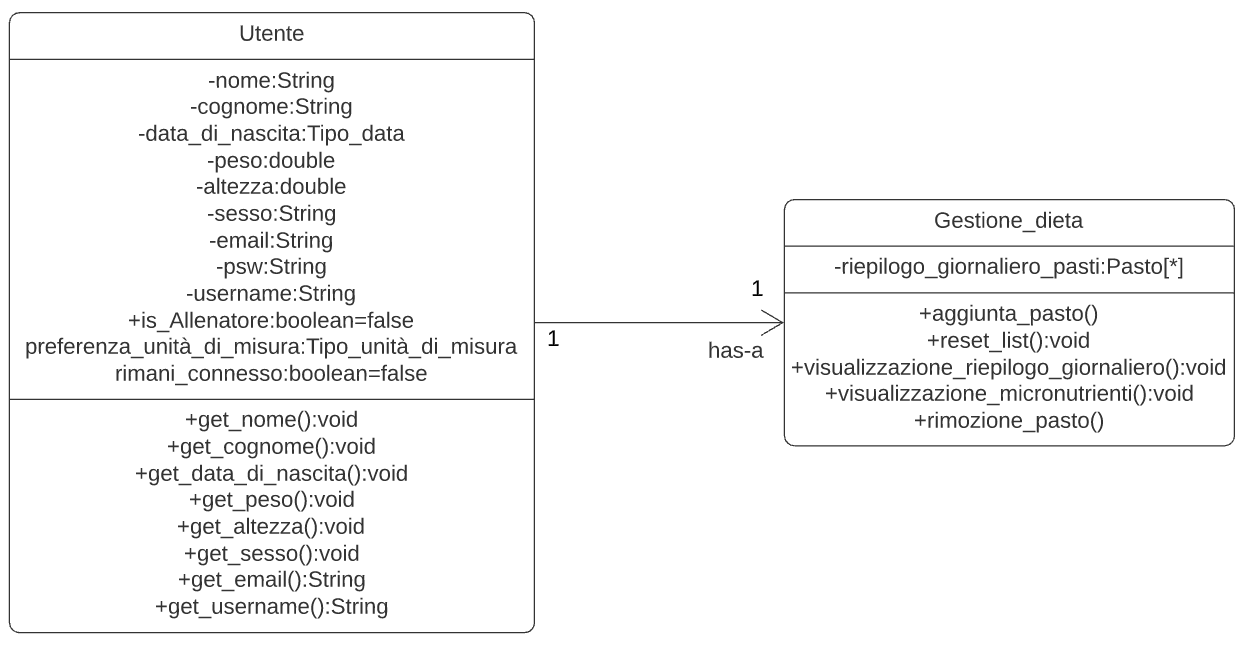
\includegraphics[scale=0.5]{classi/Gestione_dieta.png}
      \end{center}

      {\large\textbf{Gestione allenamento}}\\

      Nello studio dei componenti era stato individuato il componente “Gestione allenamento”. È stata quindi creata la classe “Gestione\_allenamento” che contiene tutte le funzioni che vanno a gestire l’allenamento dell’utente. Le funzioni presenti sono praticamente uguali a quelle in “Gestione\_dieta”.
      
      \begin{center}
            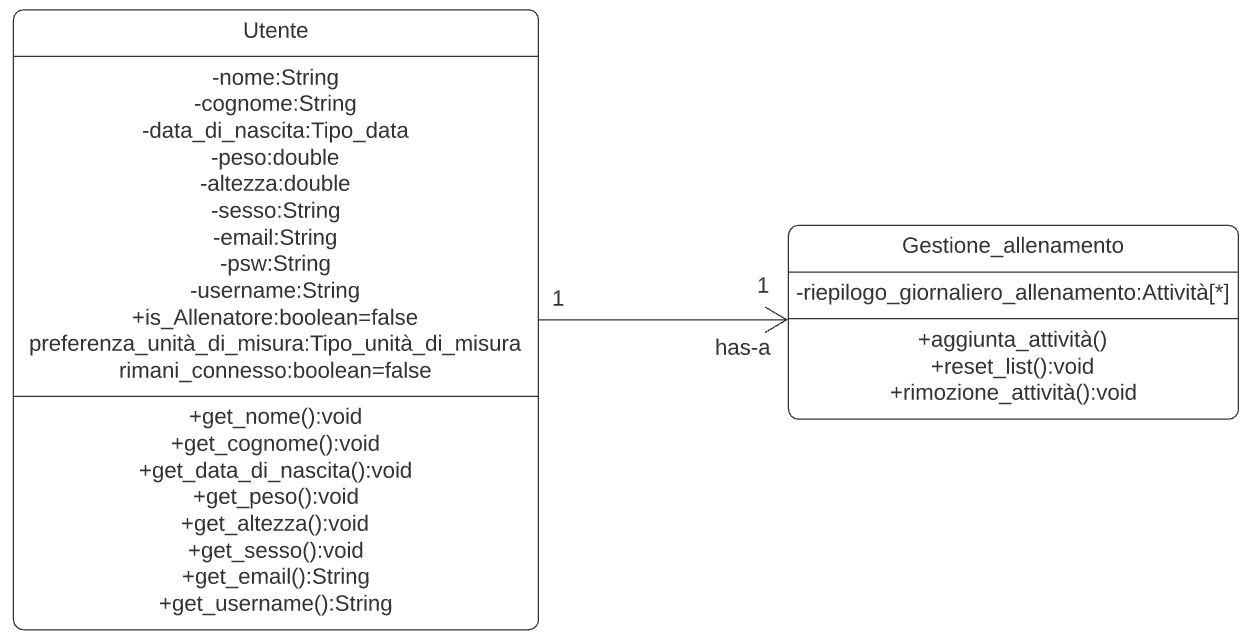
\includegraphics[scale=0.5]{classi/Gestione_allenamento.png}
      \end{center}
      
      \hfill \break
      \hfill \break
      
       \subsection{Diagramma delle classi complessivo}
    
    Di seguito viene riportato il diagramma delle classi complessivo, ovvero con tutte le classi descritte precedentemente e con i collegamenti tra esse, quando necessari.

    
    \begin{center}
        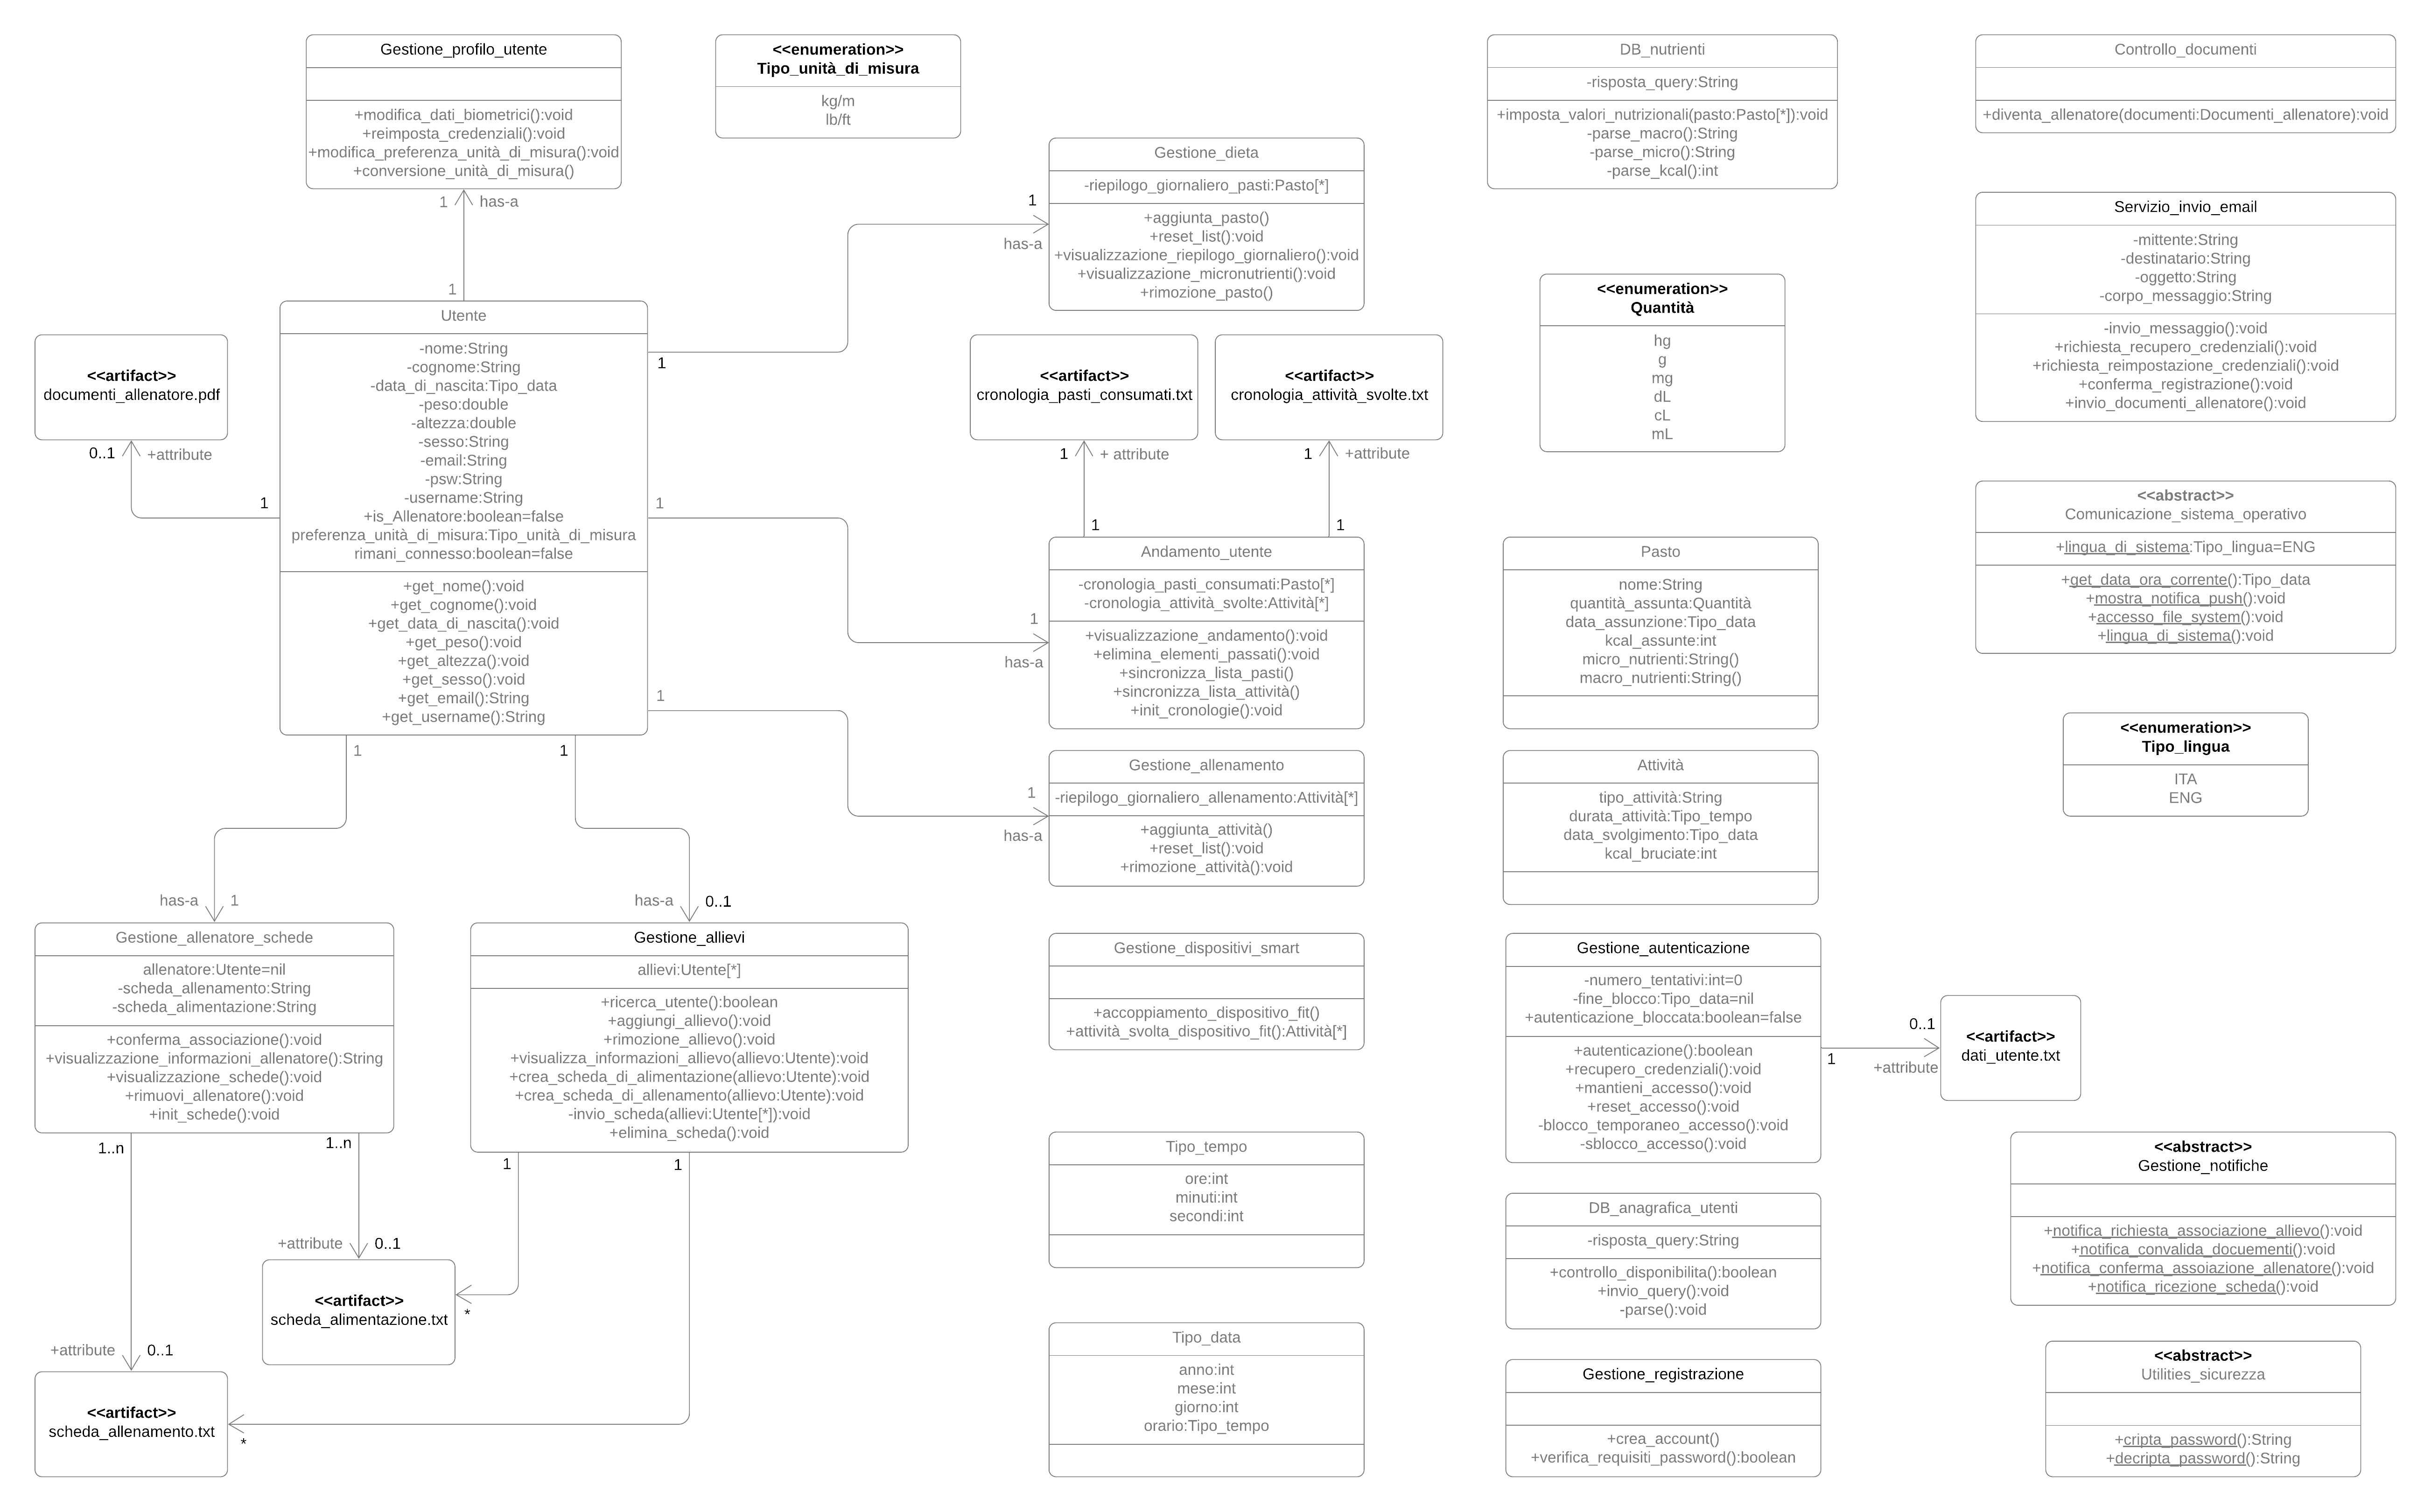
\includegraphics[width=\textheight, height=\textwidth,keepaspectratio, angle=90]{class diagram/Class diagram.png}
    \end{center}
    
    \section{Codice in Object Constraint Language} 
    
    In questa sezione descriveremo la logica prevista in alcune operazioni di certe classi. Questa logica verrà descritta in Object Constraint Language (OCL) e ricorriamo a questo strumento dal momento che non tutti i concetti sono esprimibili in modo formale in UML.\\


    
{\large\textbf{Gestione allenatore e schede}}\\


     \begin{center}
            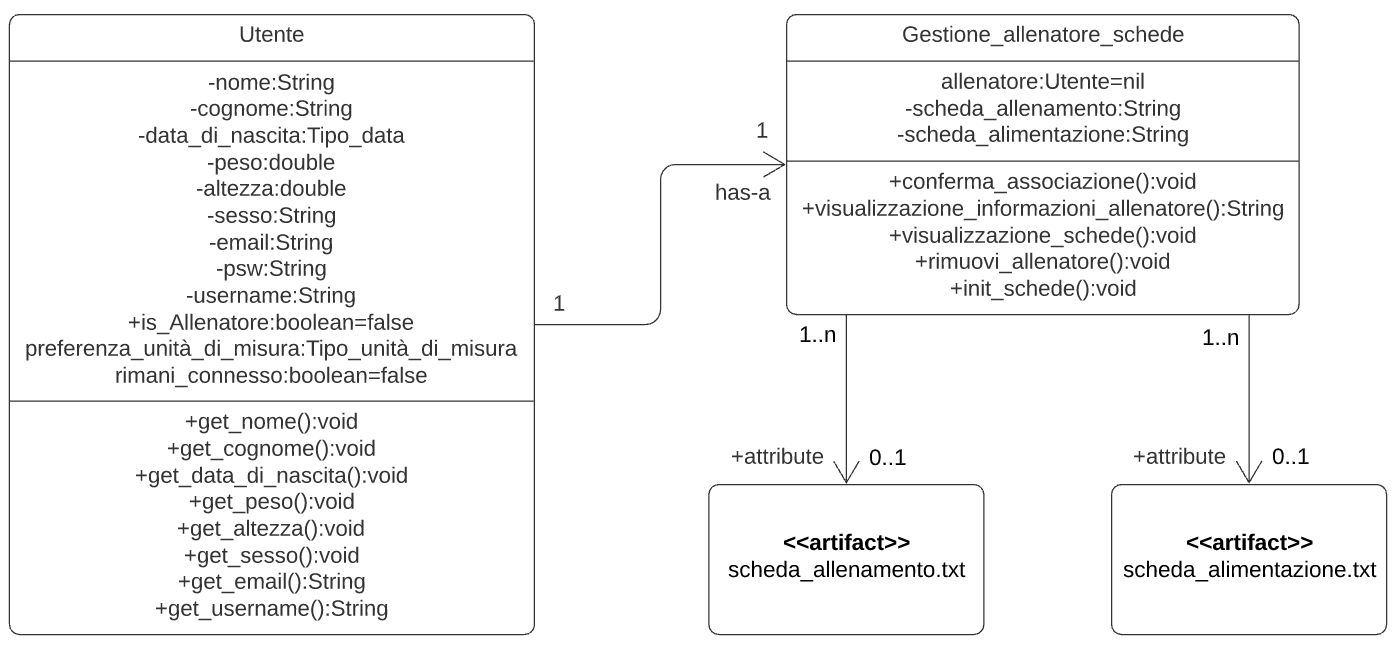
\includegraphics[scale=0.5]{classi/Gestione_allenatore_schede.png}
    \end{center}
    
      \hfill \break
      

   Un utente non può rimuovere un allenatore dalla propria lista degli allenatori se non ne ha nessuno. La condizione che un allievo debba avere un allenatore per poterlo rimuovere è espressa in OCL attraverso un invariante con questo codice:\\
   
   

    \begin{center}
            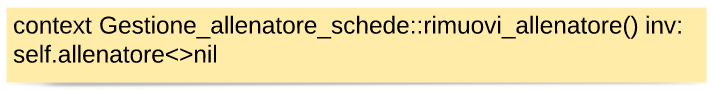
\includegraphics[scale=0.5]{OCL/Gestione allenatore e schede 1.png}
    \end{center}
    

      
      
    Un utente deve essere allenato da almeno un allenatore per poter vedere le sue informazioni. Questa condizione è espressa in OCL attraverso un invariante con questo codice:\\
    

    
    \begin{center}
            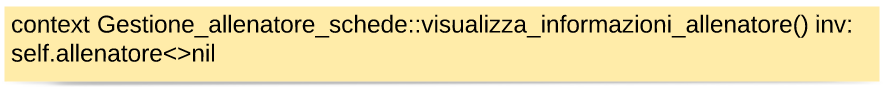
\includegraphics[scale=0.5]{OCL/Gestione allenatore e schede 2.png}
    \end{center}
    
    \hfill \break
    
    Un utente non può visualizzare le proprie schede se entrambe sono vuote. Per esprimere questa condizione in OCL si utilizza un invariante con questo codice:\\
    
    \begin{center}
            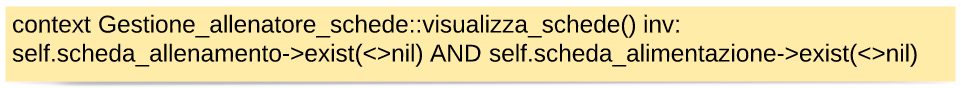
\includegraphics[scale=0.5]{OCL/Gestione allenatore e schede 3.png}
    \end{center}
    
    \hfill \break
    \hfill \break
    \hfill \break
    \hfill \break
    \hfill \break
    \hfill \break
    \hfill \break
    \hfill \break
    \hfill \break
    
    
    {\large\textbf{Gestione allievi}}\\
    
    \begin{center}
            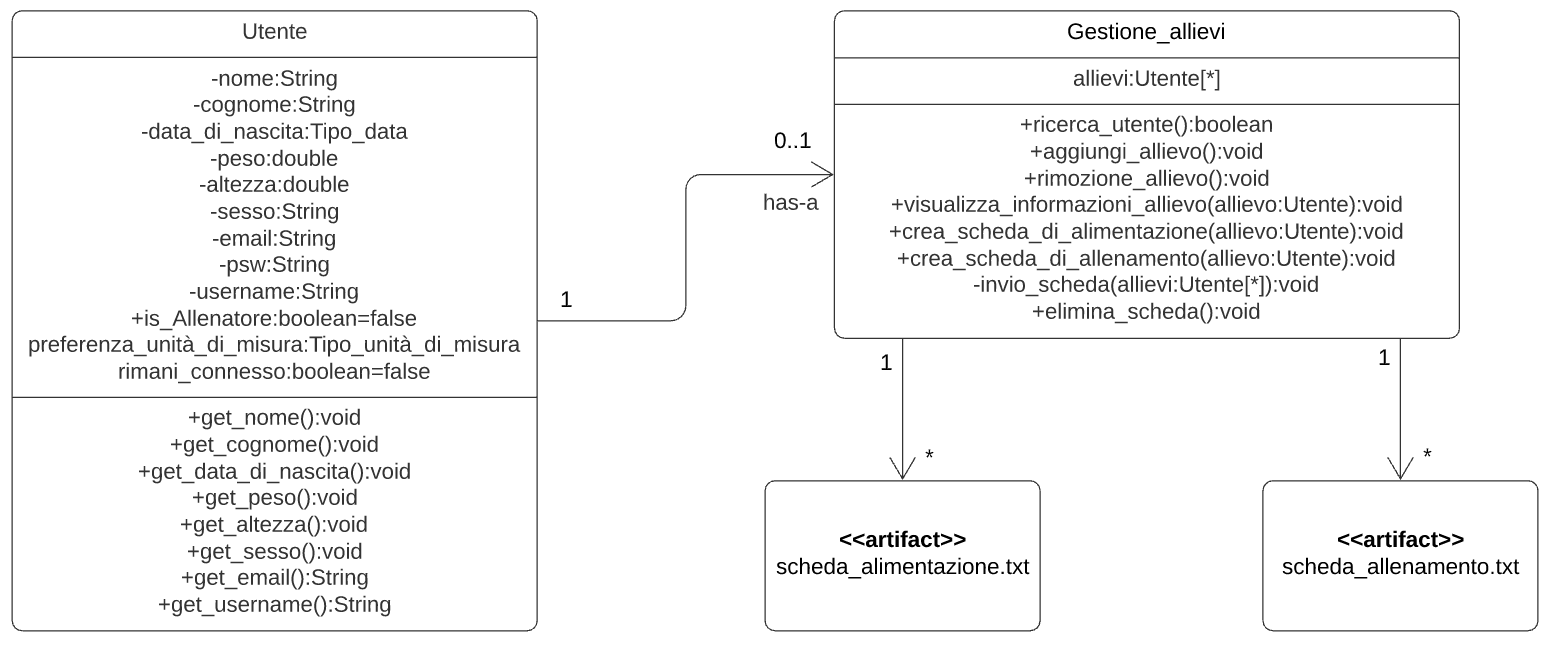
\includegraphics[scale=0.5]{classi/Gestione_allievi.png}
    \end{center}
    \hfill \break
    
    Un allenatore non può rimuovere degli allievi dalla propria lista se non ne ha nessuno. Per esprimere questa condizione in OCL si utilizza un invariante con questo codice:\\
    
    
    
    \begin{center}
            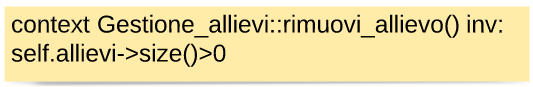
\includegraphics[scale=0.5]{OCL/Gestione allievi 1.png}
    \end{center}
    \hfill \break
    
    La classe Gestione\_allievi è ricervata a un utente che è un allenatore, quindi un utente la cui variabile di istanza is\_Allenatore è a valore true. Per esprimere questa condizione in OCL si utilizza un invariante con questo codice:\\
    
    
    \begin{center}
            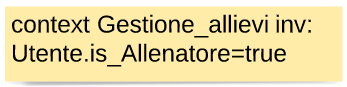
\includegraphics[scale=0.5]{OCL/Gestione allievi 2.png}
    \end{center}
    \hfill \break
    
    {\large\textbf{Utenti}}\\
    
    \begin{center}
            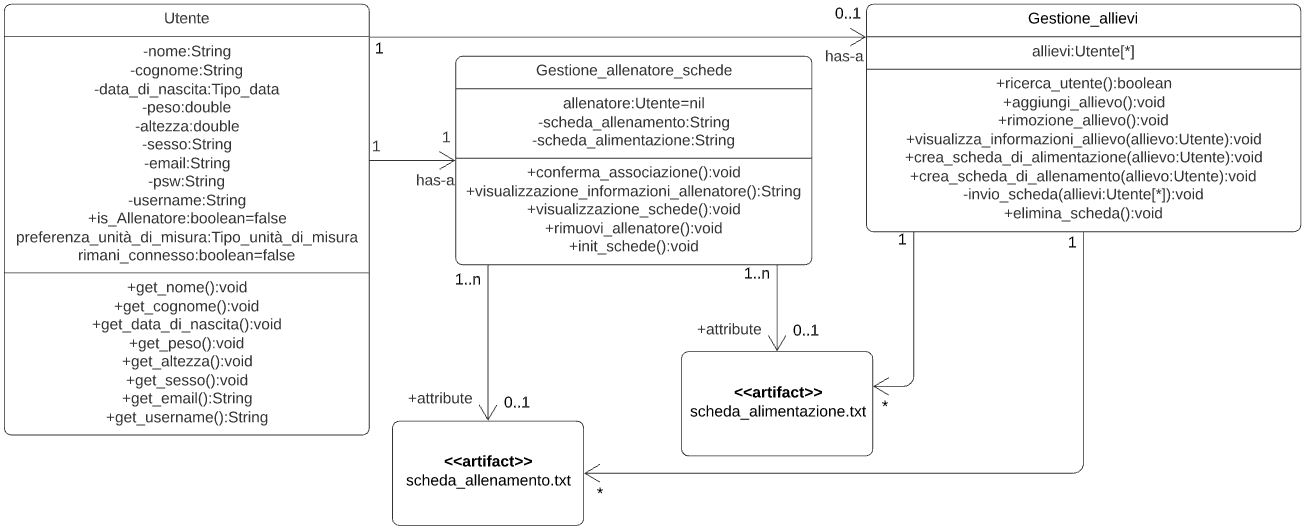
\includegraphics[scale=0.5]{classi_OCL/Utenti.png}
    \end{center}
    \hfill \break
    
    Un allenatore può utilizzare le funzioni get indicate nella casse Utente (nome, cognome, data di nascita, peso, altezza, sesso, email e username) solo se è un suo allenatore. Per esprimere questa condizione in OCL si utilizza un invariante con questo codice:\\

    
    \begin{center}
            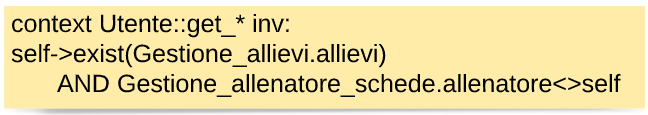
\includegraphics[scale=0.5]{OCL/Utente_nuovo.png}
    \end{center}
    \hfill \break
    
    {\large\textbf{Gestione autenticazione}}\\
    
    \begin{center}
            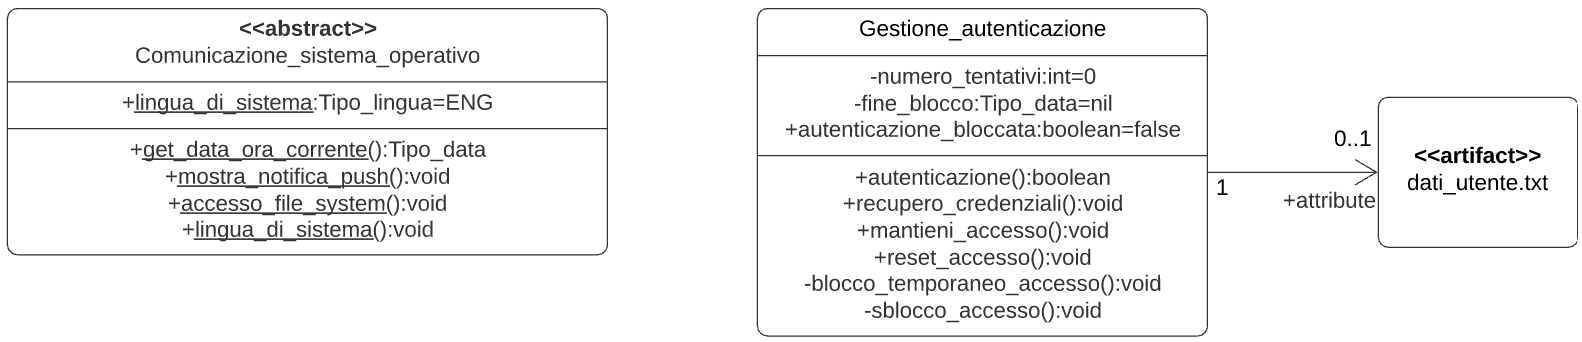
\includegraphics[scale=0.5]{classi_OCL/Autenticazione 1.png}
    \end{center}
    \hfill \break
    
    La funzione che blocca temporaneamente l’accesso all’applicazione può essere chiamata solo se ci sono stati 3 tentativi di accesso falliti. L’accesso viene in questo caso bloccato per 24 ore. Per esprimere questa condizione in OCL si utilizzano una precondizione e una postcondizione con questo codice: \\
     \begin{center}
            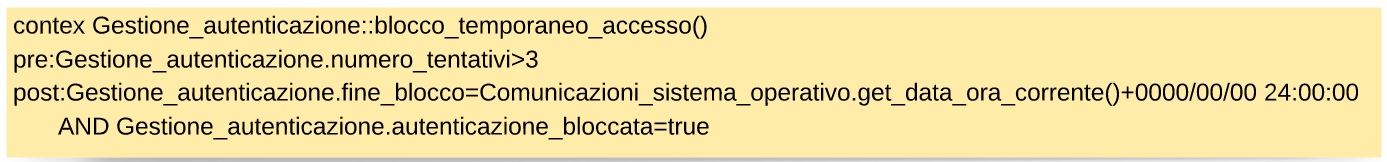
\includegraphics[scale=0.5]{OCL/Gestione autenticazione 1.png}
    \end{center}
    \hfill \break
    
    \begin{center}
            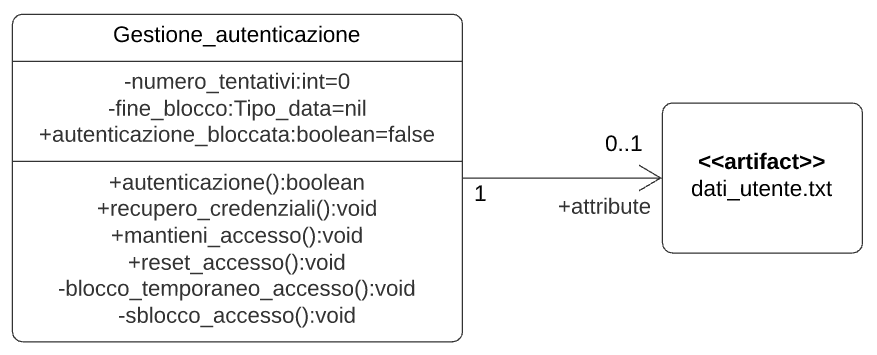
\includegraphics[scale=0.5]{classi/Gestione_autenticazione.png}
    \end{center}
    \hfill \break
    
    La funzione che sblocca l’accesso a un utente può essere chiamata solo se sono passate 24 ore dal blocco. Questa condizione è espressa in OCL attraverso una precondizione e una postcondizione con questo codice:\\

     \begin{center}
            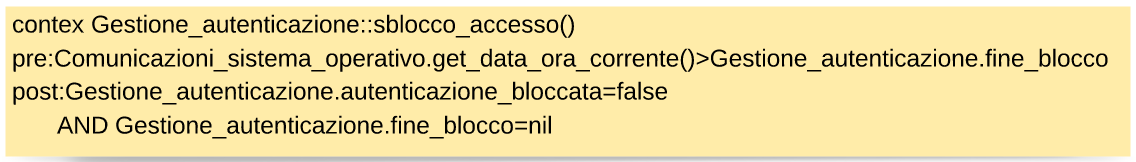
\includegraphics[scale=0.5]{OCL/Gestione autenticazione 2.png}
    \end{center}
    \hfill \break
    
    Ogni qualvolta un utente prova ad accedere, fallendo, la variabile “numero\_tentativi” viene incrementata di 1. Per esprimere questa condizione in OCL su utilizza una postcondizione con questo codice:\\

     \begin{center}
            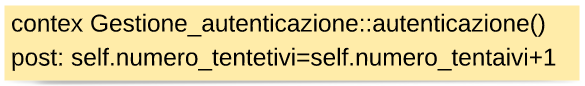
\includegraphics[scale=0.5]{OCL/Gestione autenticazione 3.png}
    \end{center}
    \hfill \break
    
    
    
    
    
    
    
    
    \section{Diagramma delle classi completo con codice OCL}
    
   Riportiamo infine il diagramma delle classi con tutte le classi fino ad ora presentate ed il
   codice OCL individuato.

\hfill \break
\hfill \break
    
    \begin{center}
        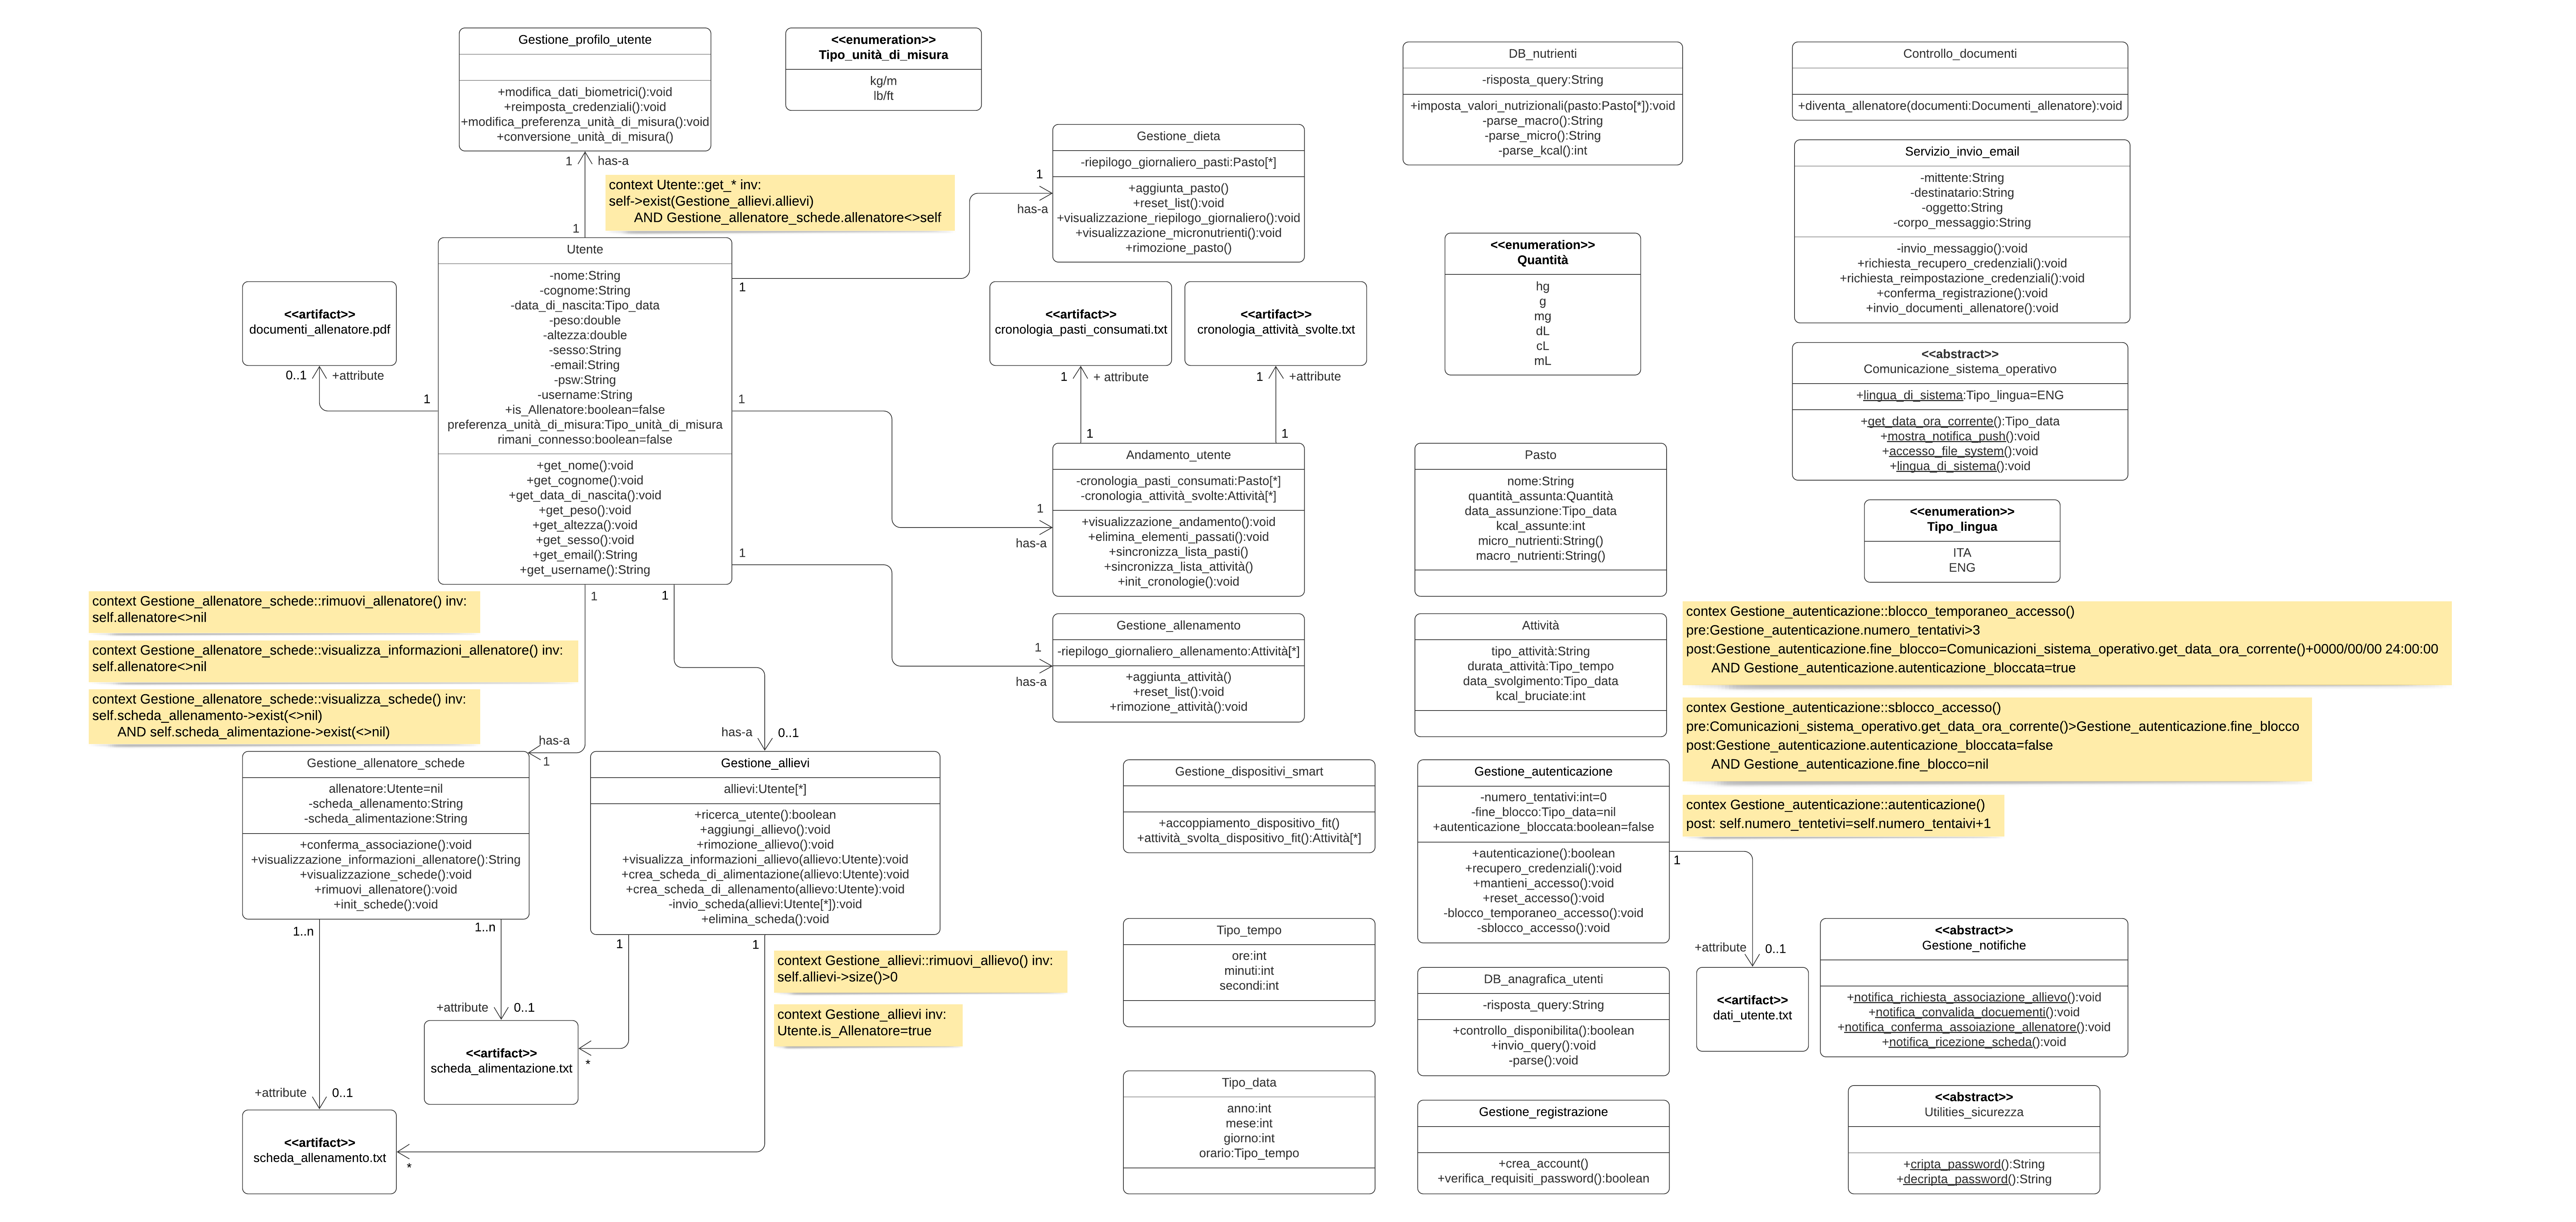
\includegraphics[width=\textheight,height=\textwidth,keepaspectratio=true, angle=90]{class diagram/Class diagram complessivo.png}
    \end{center}
    
    
    
    
      
\end{document};